\chapter{Towards Scene-Aware Acoustic Rendering Pipelines for Augmented Audio Reality}\label{ch:ar-pipeline}
The following Chapter details the implementation to address the primary objective of the thesis: proposing a scene-aware interactive rendering system for realistic sound transmissions between sound sources and a listener in AR space. The following Sections will detail how the acoustic material recognition and rendering prototypes integrate with the overarching pipeline, discussing target functionalities, design choices, limitations, and future expansions based on evaluation data obtained from evaluations provided in earlier Chapters and recent advances in the field. This Chapter breaks down into the following three areas:
\begin{itemize}
    \item \textbf{concept},
    \item \textbf{implementation}, and
    \item \textbf{vision}.
\end{itemize}
\emph{Concept} defines the proposed pipeline's architecture, objectives, and design principles; \emph{implementation} demonstrates how the pipeline can deploy to consumer HMDs as a proof-of-concept system; finally, \emph{vision} analyses limiting factors and expansion points, looking at perception factors to consider for optimisation and ablation studies.\par
Discussions on design principles, implementation, and limitations feed into methodologies for future research direction, as demonstrated by Chapter~\ref{ch:evaluation}, where the evaluation design has foundations on the outcomes of these Sections.

\section{Concept}\label{sec:overview}
In light of the work towards 
The proposed system aims to produce realistic sound transmissions between sound-emitting holograms in AR space and a listener experiencing the holograms via a head-mounted holographic display and perceived auditory stimuli via headphones. In this Chapter, the term ``listener'' is used interchangeably with the term ``user'' to refer to the user who is displayed audio-visual stimuli from both the holographic \acrshort{hmd} and the headphones. The implementation of this method for interactive sound rendering is demonstrated on a Microsoft Hololens 2 Augmented Reality Head-Mounted Headset, an embedded wearable computer with a holographic display featuring space-sensing and spatial mapping technology that enables Simultaneous Localisation and Mapping (SLAM) methods~\citep{davison2003real, ungureanu2020hololens}.\par

\begin{figure}[htb]
    \centering
    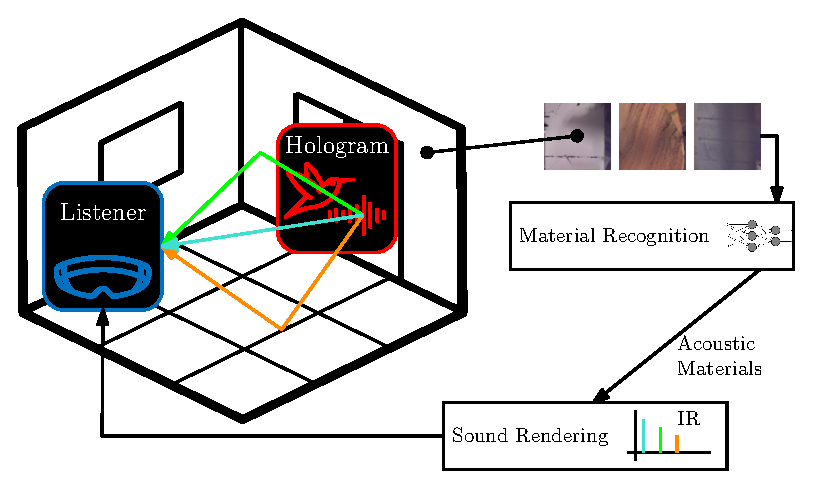
\includegraphics[width=1\linewidth]{ar-system}
    \caption[High-level diagram of the proposed sound rendering pipeline]{Overview of the presented method showing a user (blue) and listener (red) in AR space: audio-visual stimuli are displayed to the user through headphones and a head-mounted display, experiencing virtual holograms projected onto his surroundings. The proposed system aims to render sound transmissions from sound-emitting holograms and the listener realistically.}
\label{fig:method-overview}
\end{figure}

\subsection{Dynamic Environment Reconstruction}
The first link in the chain of generating realistic sound transmission between a listener and holograms in AR space is generating and handling a virtual environment to host scene elements such as virtual sound-emitting entities. In AR space, the scene geometry includes a reconstruction of the real space surrounding the user. The space surrounding the user is reconstructed using space-sensing technology featured in the Hololens 2 \acrshort{hmd}~\citep{ungureanu2020hololens}. Using the Microsoft Mixed Reality Toolkit~\footnote{\url{https://github.com/microsoft/MixedRealityToolkit-Unity}}, an environment mesh is continuously extracted as a triangulated mesh and updated every 3 to 5 seconds, reflecting dynamic changes in the environment (e.g.\ furniture being moved or a crowd entering the space).\par
The reconstructed environment mesh optimises as the user walks around the scene and can produce reconstruction errors or holes in the mesh. This technology produces reconstructions with less accuracy and precision than LiDAR scanners with dedicated hardware, such as the one used for conducting experiments in Chapter~\ref{ch:materials}, but it is still capable of producing watertight meshes, suitable for rendering applications\footnote{\url{https://learn.microsoft.com/en-us/windows/mixed-reality/design/spatial-mapping}}.\par  
The triangulated mesh, represented as a list of triangles and indices, is used to construct a \acrfull{bvh}, where triangle primitives are encapsulated in \acrfullpl{aabb}, optimising geometrical search operations for acoustic modelling such as ray-triangle intersection tests. As discussed in Section~\ref{sec:bg-geometry-handling}, One key advantage of using a \acrshort{bvh} in the pipeline is the ability to group multiple primitives in \acrshortpl{aabb} whose size can be determined by a geometry reduction algorithm to simplify the environment complexity whilst maintaining a target perceptual response from the acoustic model.\par
The \acrshort{bvh} implementation supports traversing and optimisation operations, allowing the \acrshort{bvh} tree representing the environment to support deformation and moving objects at interactive rates \citep{wald2007ray}.

\begin{figure}[htb]
    \centering
    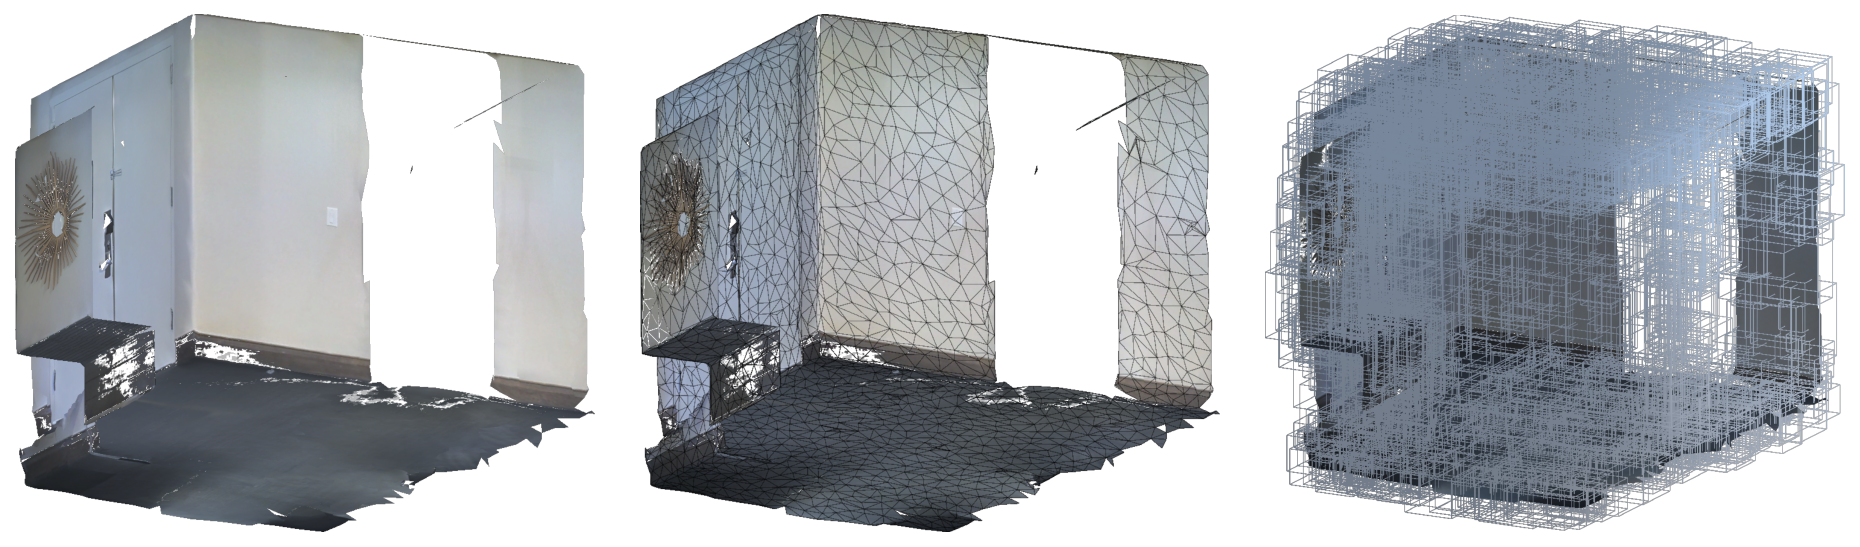
\includegraphics[width=1\linewidth]{bvh-matterport}
    \caption[A Bounding Volume Hierarchy computed on a real environment]{A visualisation of a BVH constructed on a portion of a scanned environment, left image, to demonstrate how AABBs encapsulate triangle primitives, visible in the centre image, forming a tree of boxes to partition the geometry.}
\label{fig:bvh-visualisation}
\end{figure}

\subsection{Material Tagging from Partitioned Space}
One key advantage of the employment of a \acrshort{bvh} for the handling of scene geometry is the space partitioning that can be used for the material tagging process. As discussed in Chapter~\ref{ch:materials}, \acrshortpl{cnn} offer efficient approaches to mapping the appearance of surfaces to the acoustic characteristics of their materials, like absorption or scattering coefficients. The space partitioning provided by the \acrshortpl{bvh} here is used to capture the appearance of portions of the reconstructed environment in order to determine the material characteristics of its surfaces.\par
The employment of a \acrshortpl{bvh} additionally allows the generation of ground truth data for acoustic material mapping processes: with access to the physical space, the acoustic material classification pipeline can test the accuracy of material tagging against labelled mesh segments. This would allow the pipeline to better target specific ecosystems of materials by creating sets of training data by labelling representative environments and generating image patches from the reconstructed space partitioned by the \acrshort{bvh}.

\subsection{Acoustic Rendering Pipeline}
\begin{figure}[htb]
    \centering
    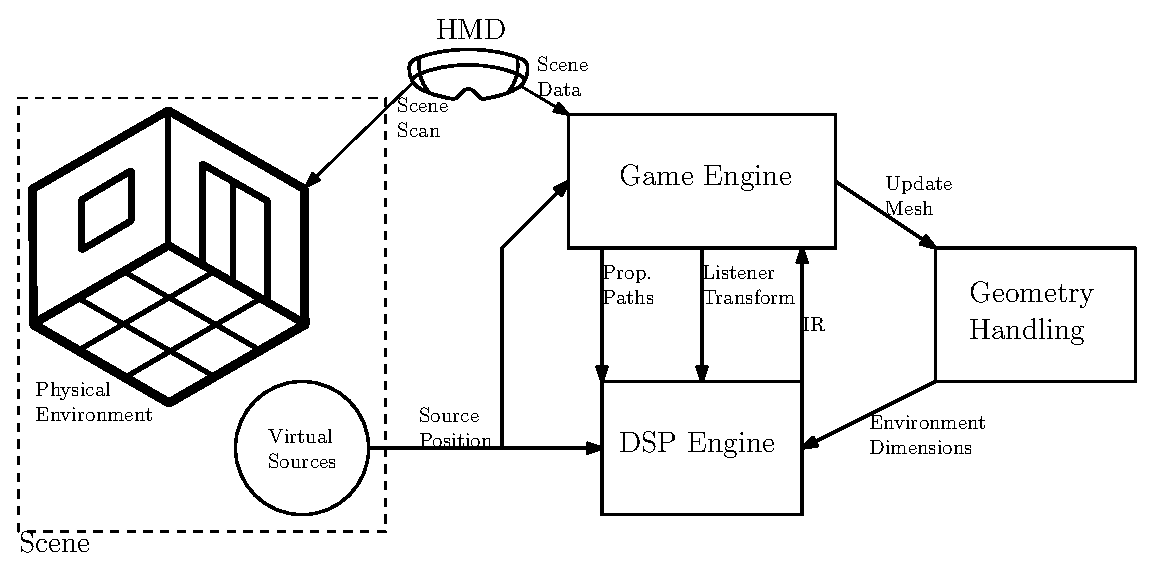
\includegraphics[width=1\linewidth]{ar-pipeline-diagram}
    \caption[Proposed acoustic rendering pipeline --- integration with game engines]{An overview of the technical implementation of the proposed pipeline for spatial audio rendering applied to an Augmented Reality interactive application. }
    \label{fig:ar-pipeline-overview}
\end{figure}

\subsection{Overview}
As discussed in Chapter~\ref{ch:lit-review}, the current state of research towards realistic auditory display in virtual environments leverages deep learning-based methods, using \acrshortpl{nn} to create latent representations of soundfields \citep{liu2022sound, ratnarajah2022mesh2ir, chen2023everywhere}. These methods often encode visual and geometrical features of the environment, as well as spatial features relating to the source and listener. These avenues are, however, experimental and require intense use of GPUs or hardware, making it hard to test on wearable computing platforms. Classic geometrical acoustics-based pipelines continue to receive attention from both research and professional domain, making ray tracing or hybrid techniques faster and more efficient by exploiting parallelisation paradigm in modern compute hardware \citep{cowan2010gpu,diaz2021gpurir}.\par
The geometry handling system provides the foundations for supporting real-time auralisations in \acrshort{ar}, as it provides a solution to the problem of defining acoustic geometry: auralisations can be produced from simplistic cuboid volume to realistic reconstructions of space with orders of fidelity to the physical counterparts of millimetres. Computational costs associated with generating auralisations rise with the number of geometrical primitives used in the reconstructed space: in triangulated meshes, detailing smaller structures in a 3D model increases the number of triangles. Detailed scene geometry allows approximation of acoustic phenomena and generally contributes to high-resolution soundfield modelling, though the computational requirements make it unfeasible for interactive applications. As discussed in Chapter~\ref{ch:lit-review}~and~\ref{ch:acoustic-rendering}, studies outline a perceptual threshold and benchmark to define the minimum level of detail required from reconstructions, and recent research on acoustic simulations conducted over the last decades has expanded towards defining what is required from a virtual environment to produce a believable simulation. Combined with advances in real-space scanning technology and user-friendly 3D reconstruction software, it is now possible to create appropriate virtual environments for acoustic simulations without requiring expert computer graphics engineering knowledge.\par

\subsection{Selecting Acoustic Rendering Techniques}
A central problem inherent in the task of interactive soundfield approximations for generating dynamic auralisations is the task of adopting a method for propagating anechoic audio in a dynamic scene. As discussed in Chapter~\ref{ch:lit-review} there are families of sound rendering techniques that produce auralisations with varying levels of realism evoked by audio propagated in the simulated soundscape and associated computational costs, as well as limitations due to their inherent architecture or nature.\par
Ray-based techniques, wave-ray hybrid techniques, and wave-based techniques have emerged as prominent methods to generate impulse responses in the field of acoustics, each contributing to understanding how sound propagates within a given space. Ray-based techniques, rooted in geometric acoustics, simulate sound by tracing rays that emanate from a source and bounce off various surfaces within a space. This method creates echoes and reverberations, contributing to the overall impulse response. Notably, it offers efficiency as it is computationally less demanding than wave-based techniques, making it suitable for real-time applications or large-scale spaces often found in cultural heritage contexts. The geometrical nature of ray-based methods allows for easier integration with existing architectural models or historical reconstructions, and the method's inherent flexibility makes it easily adjustable to different acoustic scenarios. %Bring in the context of real time RIRs
On the other hand, wave-ray hybrid techniques present a more complex picture, combining aspects of ray-based and wave-based methods. Rays are utilised to model the high-frequency components of the sound, while wave equations handle the low-frequency behaviour, attempting to capture the best attributes of both methods. However, the hybrid nature often means more computational resources are needed, and it might not always be the most suitable choice for cultural heritage applications where both high and low-frequency accuracy is not often the primary concern.  %Discuss how this fits into the prototype design
Wave-based techniques stand out for their precision, solving the wave equation to simulate how sound waves propagate through space, accurately modelling diffraction, scattering, and other complex wave phenomena. While highly accurate, wave-based techniques often require substantial computational resources, making them less suited for real-time or large-scale applications. Moreover, this level of detail may exceed what is necessary for conveying the historical or cultural experience.
Considering the landscape of immersive acoustics, ray-based techniques offer a compelling option for real-time applications and limited computational resources. Their computational efficiency, relative simplicity, and adaptability in handling various scenarios effectively capture the essential acoustic characteristics of historical spaces. Unlike wave-based or hybrid methods, ray-based techniques can prioritise the aspects most relevant to the experience and understanding of cultural heritage, aligning well with the objectives and constraints often found in this field. Therefore, while the high accuracy of wave-based methods or the comprehensive nature of hybrid methods may have specific applications in areas of cultural heritage investigations, it is the ray-based techniques (such as those employed by acoustic simulation software such as ODEON) that generally stand out as the most appropriate choice for the unique challenges and opportunities presented within the context of \acrshort{ar}.

\subsection{Real-Time Spatial Audio Rendering Techniques}
The proposed system approximates acoustic phenomena from a dynamic environment reconstructed as the user interacts and navigates the complex scene, considering physical and objective factors of the soundscape. The \acrshort{has}, however, is the final and crucial link in the chain of the reproduction system, requiring the pipeline to consider psychoacoustic and human factors in generating auditory stimuli expressed as binaural audio. The integration of factors of the \acrshort{has} and the convolution of anechoic audio completes the 3D spatial audio chain.\par
\acrfullpl{hrir} offer a compact solution to the integration of \acrshort{has} features, much like room responses, as we can convolve a monaural signal to the frequency representation of a pair of \acrshortpl{hrir} (one for each ear), the \acrfull{hrtf}. Hence, the discussed real-time convolution algorithms \citep{kim2019immersive} can be used, in combination with the $h$ \acrshort{rir} signal, to generate binaural rendered audio channels $y_{left}$ and $y_{right}$ from a monaural signal $x$:
\begin{equation}\label{eq:binaural-hrtf-example}
    y_{left} = x * \acrshort{hrtf}_{left} * h \quad \textrm{and} \quad  y_{right} = x * \acrshort{hrtf}_{right} * h \textrm{.}
\end{equation}
\acrshort{hrtf} channels left and right are evaluated in real-time, depending on the current position and rotation of the listener entity in the virtual environment, using a loaded bank or \acrshortpl{hrir} that are often real measurements of subjects across a grid of points in the azimuth and elevation surrounding the subject. These measurements record the response of each ear canal from a source position in the surrounding sphere, allowing an interactive \acrshort{hrir} algorithm to interpolate between these measurements \citep{hoene2017mysofa}.\par
Audio rendering tasks, such as performing the convolution operation indicated by Equation~\ref{eq:binaural-hrtf-example}, generally require trivial computational resources, unlike sound propagation or acoustic modelling \citep{liu2020sound}. 

\section{Implementation of an AAR Prototype System}
The following Section proposes a software implementation of the system, proposing a technical apparatus that can be employed for dynamic auralisation of sound-emitting holograms, considering approximated acoustic phenomena of \acrshort{ar} space.

\subsection{Overview}
The system, illustrated in Figure~\ref{fig:ar-pipeline-overview}, has a game engine as its core component, responsible for querying the HMD for updates on the spare surrounding the user, indexing and handling reconstructed scene geometry, computing energy transfers between emitters and receivers, and controlling a \acrshort{dsp} engine for performing audio rendering tasks.
\begin{figure}[htb]
    \centering
    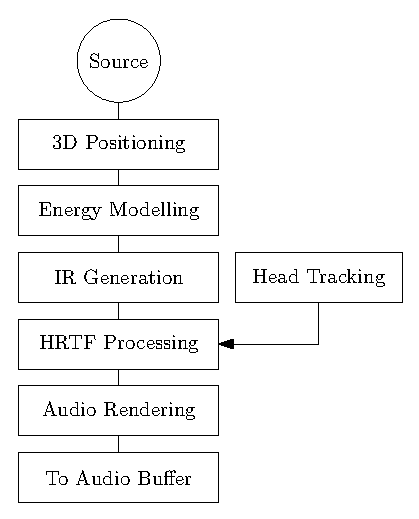
\includegraphics[width=0.5\linewidth]{source-flow-diagram}
    \caption[Flow of signal from a sound-emitting entity to rendered audio]{Rendering process of a single sound source: an input source description, positioned in AR space, is used to model its energy transfer to the listener, represented via a response function. Via head-related transfer functions based on the listener's head rotation provided by the HMD, audio from the audio is processed and sent to the output audio buffer.}
\label{fig:source-flow-diagram}
\end{figure}

\subsection{Hardware Apparatus}
\begin{figure}[htbp]
    \centering
    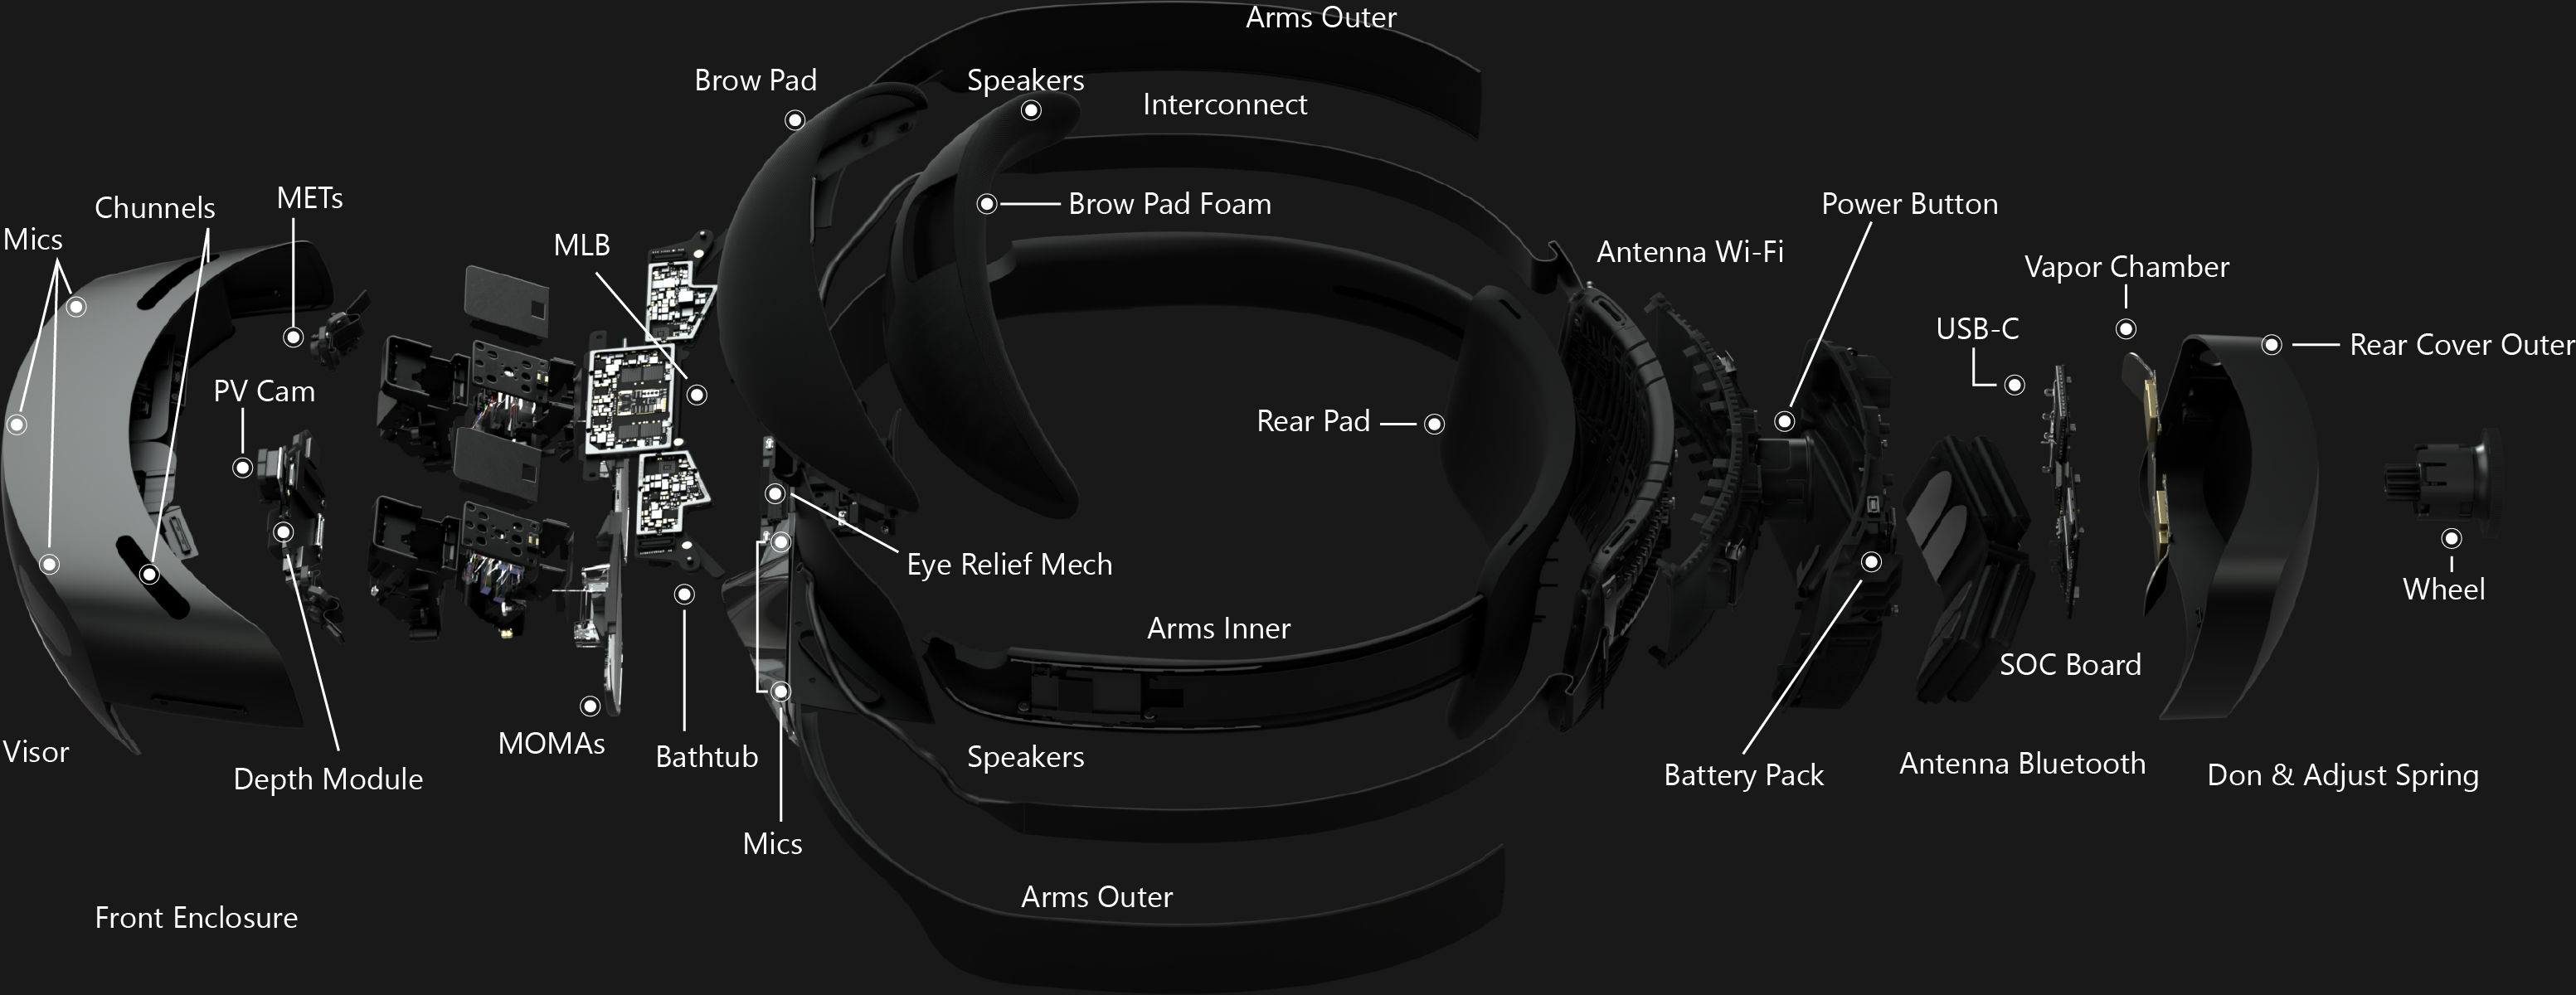
\includegraphics[width=1\linewidth]{hl2-exploded-view}
    \caption{Exploded view of the Microsoft Hololens 2 Augmented Reality Head-Mounted-Display.}\label{fig:hl2-exploded-view}
\end{figure}
This Section demonstrates the system implementation using a Hololens 2\footnote{\href{learn.microsoft.com/en-us/style-guide/developer-content/reference-documentation}{https://learn.microsoft.com/en-us/style-guide/developer-content/reference-documentation}} HMD, composed of a built-in ARM32/64 computer equipped powered by a Qualcomm Snapdragon 850 CPU with 4GB LPDDR4 DRAM.\par
As shown in Figure~\ref{fig:hl2-exploded-view}, the HMD has a visor containing holographic visual displays and featuring head-tracking sensors with four light cameras, two eye-tracking infrared cameras, 1 Megapixel depth sensor. The visual displays have $1.08mm$ focal length and $96.1^\circ$ field of view. Additionally, an accelerometer, a gyroscope, and a magnetometer allow tracking of the user's position and orientation. The device supports spatial audio reproduction with built-in speakers and a Bluetooth-connected external audio DAC. The array of sensors enables several human understanding features, such as hand and eye tracking and six-degrees-of-freedom position tracking.\par
The Hololens 2 represents a platform offering average to low computational resources when compared against the current market of \acrshort{xr} \acrshortpl{hmd}. The Meta Quest 2 \acrshort{hmd}\footnote{\url{https://www.meta.com/gb/quest/products/quest-2/}}, for instance, offers a faster Qualcomm Snapdragon XR2 CPU with 6GB of LPDDR DRAM. The overall rapid increase in compute power and memory amongst \acrshort{xr} technology sets up the proposed rendering pipeline for success.

\subsection{Game Engine and Scene Management System}
The game engine has a central role in managing operations and the lifecycle of the audio processing pipeline, as well as tracking the listener's position and orientation and managing sound sources in the complex scene. The game engine allocates computational resources to sound rendering-related operations and polls updates on the spatial reconstruction system of the \acrshort{hmd}. Hence, the design for an acoustic rendering pipeline for applications should centre around the core principles of game engine architectures.\par
Upon receiving updates from the spatial reconstruction system, whose frequency depends on the parameters of the MRTK spatial understanding setup, the game engine is responsible for updating the \acrshort{bvh} to take into account changes to the environment geometry. Here, the modularity of modern geometry handling systems, such as \cite{kopta2012fast}'s or \cite{lauterbach2009fast}'s fast and efficient implementations; designed with modularity and parallelisation in mind, allowing real-time updates and reconstruction of parts of the scene tree, making it a suitable choice for sound rendering geometry handling in \acrshort{ar}.\par
The game engine, furthermore, is responsible for the handling and positioning of sound sources, starting the source-to-listener signal flow expressed in Figure~\ref{fig:source-flow-diagram}. This includes managing anechoic audio associated with the sound source or the sound synthesis system that generates audio on the fly \citep{hamid2009review}.\par

\subsection{Engine for Spatial Audio Rendering}
\begin{table}[tbp]
    \centering
    \begin{tabularx}{1\linewidth}{lXcc}
    \toprule
    Operation                               & Inputs                                                     & Outputs & Phase   \\ \midrule
    Initialise Engine                       & Samplerate, filter kernel size, frequency bands definition & None    & Setup   \\
    Setup Block Processing                  & Chunk size, kernel size, channels                          & None    & Setup   \\
    Load HRTF Banks                         & HRTF database                                              & None    & Setup   \\
    \nohyphens{Set Energy Transfer}         & Target frequency band, data                                & None    & Runtime \\
    Render IR                               & None                                                       & None    & Runtime \\
    Process Buffer Chunk                    & Chunk                                                      & Chunk   & Runtime \\
    Update HRTF                             & Head rotation                                              & None    & Runtime \\ \bottomrule
    \end{tabularx}
    \caption{A list of operations and routines provided by the proposed DSP engine to process audio in real-time from sources depending on acoustic energy transfers and listener's orientation information. }
    \label{tab:dsptb-interface}
    \end{table}
Drawing from well-established and modern spatialiser system designs from~\cite{naef2002spatialized}~and~\cite{lakka2021x3d}, respectively, a \acrshort{dsp} engine receives control from the game engine, transforming the energy propagation modelling into binaural \acrshortpl{ir} that can propagate anechoic audio. Duties of the \acrshort{dsp} engine include manipulating signals in the time and frequency domain, requiring a fast implementation of the DTFT, and a suite of tools and routines for handling and processing \acrshortpl{ir} and transfer functions.\par
As shown in Figure~\ref{fig:source-flow-diagram}, input audio from sources undergo the time and frequency-domain manipulations based on aspects of the environment and the listener implemented by the \acrshort{dsp} engine. Table~\ref{tab:dsptb-interface} illustrates the interface to the DSP Engine, showing procedures and set-up operations to support real-time audio manipulation of sources. The set-up phase determines the sample rate for all audio manipulations, the number of points for evaluating kernel functions for filters, and the definition of frequency bands for frequency-dependent energy transfer modelling and processing. In addition, other set-up procedures include loading \acrshort{hrtf} banks from a participant record database and configuring block processing routines by specifying the current engine's audio buffer properties, such as the size of audio chunks and number of channels \citep{hoene2017mysofa}.\par
Runtime procedures, executed as the game engine runs the scene and a sound source is emitting with the listener being within the propagation radius, include setting frequency-dependent energy transfer between source and receiver, rendering a monoaural \acrshort{ir}, and processing audio emitted based on the listener's head rotation; these operations complete the chain in Figure~\ref{fig:source-flow-diagram}.\par

\subsection{DSP Engine Procedures}
A \acrfull{dsp} engine is crucial for generating spatialised audio, enabling realistic and immersive auditory experiences in immersive applications. The \acrshort{dsp} engine processes audio signals to simulate how sound propagates in a 3D environment, taking into account the positions of sound sources and listeners, as well as the acoustic characteristics of the environment. The initialisation phase is critical for setting up the \acrshort{dsp} engine with the necessary parameters and resources to perform spatial audio processing effectively. The following procedures are executed during this phase.\par

\paragraph{Intialisation}
The \acrshort{dsp} engine requires several key parameters to be configured, like sample rate, to determine the number of audio samples processed per second; or the buffer size, to define the number of audio samples processed in each block. Smaller block sizes can reduce latency but may increase CPU load, while larger block sizes can reduce CPU load at the cost of increased latency.

\paragraph{Loading HRTF Banks}
\acrshort{hrtf} banks are crucial for spatial audio rendering as they model how sound waves interact with the human head, ears, and torso. During initialisation, the \acrshort{dsp} engine loads the necessary \acrshort{hrtf} banks from external files or databases. These banks provide the filters required to spatialise audio based on the listener's position relative to the sound source.

\paragraph{Processing Audio Buffer}
At runtime, the \acrshort{dsp} engine processes audio chunks in real-time. This involves:
\begin{itemize}
    \item Applying \acrshortpl{hrtf}: The engine applies the selected \acrshort{hrtf} to the audio signals, simulating how the sound would be perceived from the listener's position;
    \item Convolving \acrshortpl{ir}: The audio signals are convolved with the pre-rendered \acrshortpl{ir} to simulate the acoustic characteristics of the environment. This step adds realism by incorporating reflections and reverberation effects.
    \item The processed audio chunks are sent to the output device (e.g., headphones or speakers) via the game engine, providing the listener with a spatialised audio experience.
\end{itemize}

Table~\ref{tab:dsptb-interface} summarises routines that compose the processing and audio signal processing of the proposed audio pipeline.

\subsection{Interactive Acoustic Rendering}
At runtime, the game engine manages operations of simulating sound propagation from a source to a listener, generating an \acrfull{rir} as a result of the operation. The implementation for this proposed pipeline leverages the work towards a ray tracing-based propagation model discussed in Section~\ref{sec:ga-based-pipeline}, underpinned by~\cite{schroder2011physically}'s work in physically-based acoustic rendering. In summary, the propagation model approximates the energy transfer from an emitter to a receiver volume, using frequency-dependent acoustic to mitigate the low-frequency limitations of geometrical acoustics modelling techniques. Given a source-receiver pair, the game engine can generate propagation a set of propagation paths for each defined frequency band, which are defined based on frequency-dependent material properties assigned to the scene geometry, which the \acrshort{dsp} engine can then use to generate a monoraural response for real-time auralisations.\par
The \acrshort{ir} generation component of the acoustic rendering pipeline is designed with a modular architecture, allowing for significant flexibility and adaptability. This modularity ensures that the system can evolve to incorporate advanced techniques as they become available, enhancing the accuracy and realism of spatial audio rendering. The modular design of the IR generation component means that it can accommodate various underlying techniques without requiring rebuilding of the entire pipeline. This flexibility is crucial for future-proofing the system and ensuring that it can integrate cutting-edge technologies as they emerge. The modular framework supports the integration of different propagation techniques, ranging from traditional geometrical acoustics approaches to deep learning methods.\par
Methods like~\cite{Singh_2021_ICCV}'s Image2Reverb can approximate reverb based on visual representations of the environment, leveraging neural networks to predict acoustic properties from images but do not consider source-listener position information within the scene and may introduce inaccuracies to the generated auralisations. Ray tracing, despite the low-frequency limitations, can still approximate basic occlusion phenomena \citep{savioja2015overview}. Though, on the other hand, upcoming \acrshort{naf}-based will be able to consider source-listener effects and generate responses at interactive rates \citep{luo2022learning}. These models can potentially adapt to dynamic changes in the environment and provide real-time soundfield simulations, ensuring that the spatial audio remains accurate as the scene evolves. Additionally, neural networks can potentially overcome the limitations of ray tracing at low frequencies by learning to model diffraction and scattering effects directly from data.\par

\subsection{Audio Rendering}
Approximated acoustic phenomena expressed in IRs are often applied to anechoic, unpropagated audio by application of the convolution operation, as discussed in Section~\ref{sec:real-time-conv}. The resulting auralisation targets a sound reproduction system by applying responses to model characteristics of a human listener in the sound field.\par
Audio rendering describes operations related to such tasks, requiring \acrshort{dsp} algorithms for real-time auralisation of audio signals from sources in a complex scene. The apparatus can display audio stimuli as a stereo signal via headphones connected to the master bus output of the game engine. The audio rendering implementation for the system needs to consider modelled source-receiver acoustic characteristics and apply spatialisation effects expressed as \acrshort{hrtf}, inserting a spatialised system in the sound reproduction chain \citep{liu2022sound}.\par
Real-time acoustic effects apply to audio buffers from scene sources via real-time \acrshort{dsp} convolution algorithms such as Overlap-Save or Overlap-Add. The former optimises the number of convolution operations. Though, this is unfavourable when the kernel function is updated frequently, leading to audio artefacts caused by outdated convolutions applied to the audio buffer. Hence, the implementation adopts the Overlap-Add algorithm, allowing for fast convolution of kernel functions, which can be updated across update calls within the engine audio thread to audio buffer chunks.\par
Figure~\ref{fig:overlap-add} shows the algorithm implementation considering \acrshortpl{hrtf} combined with \acrshort{rir} applied to a given audio signal block from the audio buffer associated with a given scene source, showing the system as a single channel for simplicity. For each update call in the engine audio thread, the algorithm convolves a block of audio samples of length $B$ containing interleaved stereo signal to a kernel function of length $K$. Zero padding, applied to both the kernel function and blocks, allows a DFT toolbox to multiply the spectrum of the two signals ($\bigotimes$ operation), generating a $B+K-1$ convolution result. $B$-long blocks (the turquoise blocks) from past convolution results sum into a new block, discarding already summed blocks (the grey blocks). Finally, the new block replaces the given input block from the audio buffer.\par

\begin{figure}[htb]
    \centering
    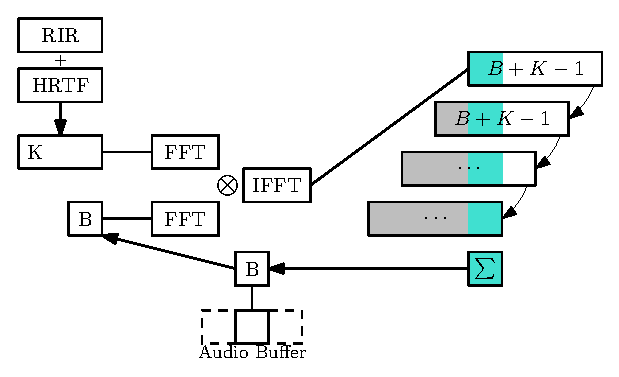
\includegraphics[width=1\linewidth]{overlap-add}
    \caption[Real-time convolution algorithm based on the Overlap-Add technique]{Overlap-Add algorithm used for real-time convolution of a kernel function expressing Room Impulse Responses and Head-Related Transfer Functions applied to chunks of audio data from an audio buffer.}\label{fig:overlap-add}
\end{figure}

\subsection{Acoustic Geometry Handling}
The geometry handling system within the acoustic rendering pipeline plays a crucial role in accurately representing the physical environment to facilitate realistic sound propagation. Environment meshes obtained from the spatial understanding system of the HoloLens Mixed Reality Toolkit, the system can effectively process geometry by constructing a \acrshort{bvh} and integrating material classification for enhanced acoustic rendering.\par
The MRTK provides detailed environment meshes that serve as the primary input for the geometry handling system. The geometry handling system constructs a \acrshort{bvh}. This hierarchical structure encapsulates the triangles from the Environment Mesh into a series of nested nodes, enabling rapid traversal and intersection testing. The \acrshort{bvh} is constructed by grouping nodes based on their spatial proximity, creating a tree where each node represents a subset of triangles of the input mesh. According to \cite{pelzer2010frequency}'s work, the minimum size for leaf nodes is set to \qty{7}{\cm} to prevent the construction of nodes that are too small to have a significant impact on the auralisation process.\par
In addition to encapsulating geometric data, nodes within the \acrshort{bvh} are used to generate image patches that express the visual features of the environment, which are essential for the material classification process. This allows the prediction of acoustic characteristics of different surfaces within the environment. For each node, the system captures visual features by generating image patches that represent the appearance of the surfaces contained within the node. These patches provide a visual context that is crucial for accurate material classification. Following the methodologies presented throughout Chapter~\ref{ch:materials}, the generated image patches are fed into a material classifier, which uses machine learning algorithms to predict the acoustic properties of the surfaces. The classifier analyses the visual features to determine attributes such as absorption coefficients.
Once the material classifier has predicted the acoustic characteristics of the surfaces, these attributes are assigned to the corresponding triangles within the \acrshort{bvh} leaf nodes. This process ensures that each surface in the input mesh is accurately represented in terms of its acoustic properties, allowing for realistic propagation modeling. The predicted acoustic characteristics are attributed to the triangles within each leaf node, enabling the DSP engine to account for variations in surface materials during the sound rendering process.

\section{Vision for Dynamic Auralisation Systems}
This section outlines the design of future prototypes for dynamic auralisations expanding from the proposed systems toward real-time interpolation of RIRs computed across a given environment. 
Beyond a baseline prototype for modelling acoustics of AR environments are potential avenues expanding towards areas of AAR. These can branch into domains of psychoacoustics and interactions between AR sound sources and listeners, adding to the overall aural experience beyond colouring ``dry'' propagating audio with acoustic effects, thus enabling the further potential for rich auditory displays in applications. Prior to expanding from the primary objective of rendering virtual audio-emitting entities that perceptually belong to the user's physical surroundings, there must be a standardised rendering pipeline that satisfies the minimum psychoacoustic requirements, as there is still a need for research defining thresholds and just noticeable differences of perceived aspects of soundfields, like reverberation or definition \citep{yang2022audio}.\par
Chapter~\ref{ch:evaluation} demonstrates a prototype deployment of the implementation discussed in the previous Sections, characterising the psychoacoustic factors associated with approximating the soundfield surrounding the user. The implementation focuses on a single sound source, omitting optimisations that target multiple sources, real-time aspects, dynamic environments scenarios, and factors targeting realistic acoustic rendering. With the human listener being the target for the generated audio-visual stimuli, rendering procedures affecting the perceived quality require probing of human perception to measure performance aspects and realism of the system. \par
Despite the need to outline perceptual responses and characterise psychoacoustic factors of rendering pipelines, a vision for research directions and expansions toward context-aware and realistic auditory interactions in AR should be developed.

% \subsection{Psychoacoustic Characterisation of Acoustic Rendering}
% A crucial aspect associated with the vision of a real-time system is defining the need to outline the minimum required threshold for realism in IRs.
% Dolhasz threshold definition \citep{Dolhasz_2020_CVPR}. 
% By reviewing a large body of work around sound rendering for \acrshort{ar}, \cite{yang2019audio} highlight the need for definitions of \acrshortpl{jnd} and thresholds for realism and presence evoked by auditory displays. 



\subsection{Combining Reinforcement Learning With Material Tagging}
Tagging materials in \acrshort{ar} space has been shown to significantly influence simulated soundfields and resulting auralisations. By accurately identifying and assigning acoustic properties to surfaces within an \acrshort{ar} environment, it is possible to create highly realistic and immersive auditory experiences. This process involves matching virtual acoustic materials to their physical counterparts and validating the accuracy through impulse response measurements. The precision of material tagging directly impacts the quality of sound propagation and the user's overall auditory experience.
So far, this work has primarily focused on matching virtual acoustic materials to their physical ground truth, especially considering the work in Chapters~\ref{ch:materials} and~\ref{ch:acoustic-rendering}, involving testing to ensure that the virtual materials accurately replicate the acoustic properties of the real-world surfaces they represent. The error margins are assessed based on impulse responses measured from the physical environment, aiming to minimise discrepancies and enhance realism.\par
Reinforcement Learning (RL) offers tools that can target wider problems around \acrshort{xr} and fields of acoustics by leveraging material tagging. Rather than achieving the closest match between virtual and real acoustic materials, RL agents can be trained to assign materials to geometry within a given environment to improve the parameters of its soundfield. RL agents combined with simulated soundfields are being explored as part of new research avenues around audio-visual navigation or locomotion for robotics applications, where models can be trained to understand acoustic characteristics or space by analysing visual and geometrical features of virtual environments \citep{chen2021semantic, gan2020look}.
The training process would involve simulating various configurations of acoustic materials and evaluating their impact on the impulse response. The RL agent uses this feedback to iteratively adjust the material assignments, gradually converging on an optimal solution that meets the target criteria.
The application of this has several practical benefits and potential use cases around architectural design, achieving specific acoustic properties is crucial for spaces such as concert halls, recording studios, and lecture theaters. An RL agent can predict and select materials that optimise sound quality, ensuring that the designed spaces meet the desired acoustic standards such as ISO standards for assessing acoustics of space for musical performance. This is an open research avenue that has been explored using classic sound rendering methods by \cite{funkhouser2004beam} and \cite{heimes2019real}.


\subsection{Hear-Through Displays and Context-Aware Dereverberation}
Among the requirements and design principles of audio pipelines are safety and accessibility; the platform should interact with the user's safety and improve their perception of their surroundings. \par
An important task here is improving the perception of physical sound sources through dereverberation techniques, leveraging scene understanding techniques and human-computer interfaces to resolve the cocktail party problem in adverse acoustic environments with concurrent propagating sources. A real-time system to improve perception of physical sound sources in AR space could target hard-of-hearing users to increase intelligibility and reduce information loss in sound transmissions, targeting a range of use cases around accessibility, training, or education. \par
Speech dereverberation is still an open research question in signal processing domains where the primary task is to perform signal processing to reduce the impact of the environment on a given sound transmission. Modern approaches to dereverberation extract features from a given signal, as demonstrated by~\cite{santos2018speech}, understanding characteristics of the soundfield in which the signal propagates to counteract the colouring effects responsible for reverberation and other acoustic phenomena affecting the unpropagated sound, which hinder definition, clarity, and intelligibility and can render auditory information inaccessible to some users.\par
Speech dereverberation techniques directly benefit from advances in sound rendering algorithms targeted at AR as they allow reconstructions of characteristics of soundfield for arbitrary placements of sources and receivers, as well as architectures and materials of the environment. This information provides dereverberation algorithms with knowledge about a sound transmission and an RIR that can counteract the colouring affecting the signal, enhancing clarity and definition by recovering the unpropagated signal.\par
\cite{chen2023learning} demonstrate an example implementation using a multimodal DNN with RGB images, depth maps, an input audio signal, and a processed de-reverberated signal as output. Their system can remove reverb and recover characteristics of the soundfield across a set of large-scale 3D reconstructions of physical environments. AR platforms provide sensing technologies to satisfy the input of such example systems. A vision for audio pipelines should consider these processing techniques as AR scenes become increasingly complex and able to interact with physical entities surrounding the listener.\par
A crucial use case for this avenue would be creating accessible applications for improving speech intelligibility in noisy environments. For instance, receiving information from a tour guide in a museum, speaking may be a challenging task for some due to the highly reverberant environment affecting the clarity and definition of the sound transmission between the tour guide and the recipient. Here, a dereverberation model can leverage hear-through displays by:
\begin{itemize}
    \item registering the tour guide as a sound-emitting entity within the \acrshort{ar} space and capturing their audio;
    \item simulating the acoustic soundfield based on the reconstructed physical environments obtained by the spatial understanding system;
    \item applying dereverberation to the captured audio from the tour guide, based on the simulated soundfield;
    \item presenting the processed audio with improved clarity and definition to the user to complete the hear-through display system.
\end{itemize}

\subsection{Extension to multiple sources and source clustering}
There is potential for sound rendering for large multi-source scenes, leveraging the work presented by~\cite{schissler2016interactive}; the authors introduce a novel sound rendering method that can handle from a few hundred to thousands of sound-emitting objects using ray tracing-based renderers. A factor to consider in the proposal of novel audio pipelines is how rendering processes are limited to the number of sound sources they can manage in a dynamic complex scene. Their method achieves this with a perceptual metric-driven source clustering paradigm based on the premise that sound sources that distant or occluded emitters can be perceptually difficult to distinguish. Thus, the audio engine can approximate multiple emitters as one, provided there is a line of sight among clustered emitters, i.e., no occlusion across emitter pairs.\par
As virtual complex scenes become increasingly rich in entities and more dynamic, source clustering is a psychoacoustic-related factor important to perceptual rendering. Audio pipelines can increase their efficiency by applying selective rendering in busy scenes, often essential for realism and optimal performance of generation of audio-visual stimuli for training applications and simulated realistic environments \citep{Woodward2021}. Hence, source clustering should be considered when designing novel pipelines by probing human perception to outline perceptual thresholds and evaluate how well listeners are able to distinguish individual sound sources in complex environments with concurrent source clusters.\par

\subsection{Extension to Dynamic Impulse Response Interpolation}\label{sec:dynamic-rir-expansion}
Recent advances in CNNs enable image-to-image networks to infer characteristics of a given soundfield. \cite{Singh_2021_ICCV} present pioneering work by proposing a novel network that infers an RIR from a single RGB image describing an environment where a hypothetical sound transmission occurs. They use image-to-image CNNs due to their ability to extract features from visual representations and map those to a latent space that can project onto an image expressing the frequency domain of an IR. The single input image expands into an RGBD image using a state-of-the-art depth prediction network \citep{bauer2021nvs}, which provides insights into the architectural features of the space described by the input image. Their method can predict reverberation features of a given space and has the potential for sound rendering and dereverberation applications in AR platforms. Furthermore, such a system has promising performance and efficiency metrics thanks to the task of understanding and prediction sound transmissions within a soundfield compresses into a forward pass of a neural network, which is becoming more trivial by the year, as both tensor processing hardware provided in consumer platforms optimises for such operations and cloud computing becomes more ubiquitous.\par
One limitation, however, is the omission of source-listener position pair information considered in the reverberation estimation process, resulting in an IR agnostic of some crucial factors of sound transmissions. There is the potential for expanding this system to provide a more accurate output by considering the position of the hypothetical source and listener in AR space. The method proposed by~\cite{Singh_2021_ICCV} could leverage depth estimation and scene understanding paradigms provided by the AR platform to provide information about the listener's position and orientation, the source position. The expanded network would combine visual and spatial features to understand acoustic phenomena affecting transmissions beyond reverberations, such as occlusion or diffraction. The network's training process would leverage artificial soundfields based on real environments by creating datasets expressing a range of sound transmissions affected by such acoustic phenomena. The work by~\cite{chen2022soundspaces} is becoming a pillar of modern sound rendering, thanks to the ability to simulate such acoustic phenomena in realistic environments that enable multi-modal perception. A vision for sound rendering AR should leverage the potential of such DNN-based approaches to infer characteristics of soundfields with high efficiency, sidestepping the computational load of using geometrical acoustics or other classic propagation techniques.\par

\subsection{Extension to Radiance Fields for Inferring Local Acoustic Features of Reconstructed Space}
Parametric soundfield coding for interactive applications, as recently advanced by~\cite{raghuvanshi2018parametric}, provides an efficient solution to real-time auralisations in complex scenes and game engines, allowing simulations of advanced acoustic phenomena by leveraging wave-based sound propagation techniques.
Even more recently, building upon the domain of neural radiance fields, the pioneering work from~\cite{luo2022learning} proposes novel neural acoustic fields able to represent the soundfield of arbitrary complex scenes. Their \acrshort{naf} takes parameters of source-receiver positions pairs, as well as listener's orientation information, to produce a function that represents a \acrshort{rir} as a \acrshortpl{stft} that can be represented as a time-domain response. The \acrshort{naf} can train by comparing generated spectrograms, using an \acrshort{mse} loss function against ground-truth counterparts from synthetic or real datasets \citep{chen2022soundspaces}.\par
\acrshortpl{naf} learn using joint acoustic/visual representations to construct a local geometric grid that can infer acoustic energy transfer from emitter to receiver by querying the radiance field. The technique performs feature extraction on a triangulated environmental mesh, modelling reflection, occlusion, and other soundfield phenomena represented by a volumetric scene function. Similar to wavefield coding techniques, \acrshortpl{naf} suffer from requiring training every time the state of the environment has changes that may have perceptual responses in the resulting auralisations, such as new holograms introduced to the complex scene or moving objects in the physical space, causing the feature grid to be outdated. The technique should be able to update segments of the feature grid by computing inference on the updated spatial reconstruction mesh provided the \acrshort{hmd}.\par
Here is a potential alternative to leverage the feature extraction process, discussed in Section~\ref{sec:dynamic-rir-expansion}, using an image-to-image network to infer characteristics of the soundfield from visual descriptions of the environment. \acrshort{ar} platforms offer arrays of cameras that can describe the environment surrounding the user. With image-to-image networks inferring acoustic properties of space photographed as the user looks around, it would be possible to project such features onto a grid that can be queried to produce acoustic responses. The benefit of such expansion would lie in the implementation of a system that continuously updates feature points, providing an online grid that can reflect dynamic changes to both the virtual and physical environment.\par
Even by employing radiance fields, the interface between the game engine and the \acrshort{dsp} engine would be maintained valid as the game engine would query the radiance field based on the current source and listener position.

\subsection{Conclusions}
Design principles and potential research avenues are identified to provide a vision that leverages the potential provided by \acrshort{ar} platforms around sensing technologies shipped with consumer hardware and interfaces with the user and the physical world. This vision reflects on a base prototype expressed as a system composed of individually tested components to achieve several goals associated with standard audio pipeline design standards. This Chapter has shown how several research domains could benefit from expansions stemming from the prototypes and addressing tasks associated with use cases such as accessibility or enhanced perception of surroundings around users wearing \acrshort{ar} \acrshortpl{hmd}.\par
Given the early stage of the prototype, the next step towards an end-to-end deployable solution should consider testing and the analysis of human factors, evaluating how the components discussed and developed so far work together to produce auditory stimuli with improved realism and presence compared to standard audio implementations in game engines. This should generate insights into the feasibility of the overall pipeline and provide data on the perceptual aspects. Chapter~\ref{ch:evaluation}, following from this, will illustrate and discuss preliminary subjective testing with an offline deployment of the proposed pipeline.
